%
% LaTeX report template 
%
\documentclass{article}
\usepackage{graphicx}
\usepackage[english]{babel}
\usepackage[latin1]{inputenc}
\usepackage{hyperref}
\usepackage{underscore}
\usepackage{amsmath}
\usepackage[english]{babel}
\usepackage{graphicx}
\usepackage{amsmath}
\usepackage{listings}
\usepackage[justification=centering]{caption}
\usepackage{float}

\topmargin=-0.45in
\evensidemargin=0in
\oddsidemargin=0in
\textwidth=6.5in
\textheight=9.0in
\headsep=0.25in

\linespread{1.1} % Line spacing
%
\begin{document}
%
   \title{Machine Learning Final Project Report}

   \author{Yu Zhang, yzhan007@odu.edu\\  Udochukwu Nweke, unwek001@odu.edu}
   
   \date{December 14th, 2018}

   \maketitle
   
 
  \newpage
    
% This is a comment: in LaTeX everything that in a line comes
% after a "%" symbol is treated as comment


   \tableofcontents
   
     \newpage
     
     
    \textbf{ \abstractname{}}\\
    
\noindent Random forests have become one of the most successful models used in data mining and machine learning because of their amazing accuracy and effectiveness. Despite their extra ordinary accuracy and effectiveness, they are primarily limited to multidimensional data because they sample features from the original data sets. In this report, we have reviewed and implemented a method that is an extension of random forests and this model works with any arbitrary set of data objects as long as similarities can be computed among data objects. It is well known that similarity computation between all $O(n^2)$ pairs of n objects can be computationally expensive, the method proposed in the paper computes only a small fraction of the $O(n^2)$ pairwise similarities between objects to construct forests. Similarity forests approach have proven to efficient and accurate on a wide variety of data sets. Hence, similarity forests extends the applicability of random forests models to arbitrary data domain. In most cases, similarity objects between objects are not completely specified because of the difficulty in collecting such values. Similarity forest can be used in these cases with straight forward modifications. \\

    
 \newpage
\section{Introduction}
Decision trees models are used for both classification and regression models. they are used to anser a sequential questions which goes down a certain route of tree given the answer. Decision trees model uses the ``if tis and that'' conditions ultimately yielding a specific result. Figure  ~\ref{fig:decisiontree} explains how decision tree works. The outlook has one of three options: sunny, overcast, or rainy. The tree shows how many questions are asked before reaching a predicted classification.\\

Decision tree has its advantages and disadvantages. some of the advantages are: 
\begin{itemize}
\item Decision trees are easy to interpret and make straightforward visualizations.
\item  The capability of the internal workings being observed makes the work easy to reproduce.
\item The can perform in both numerical and categorical datasets, and they are extremely fast.

\end{itemize}
Some of the disadvantages are:
\begin{itemize}
\item Decision trees require an algorithm capable of determining an optimal cjoice at each node. 
\item Decision trees are prone to overfitting. This happens when the tree is particularly deep. this is as a result of the amount of specificity looked at, leading to smaller sample events. These small samples may lead to unsound decisions.
\end{itemize}
 The ideal thing would be to minimize both error due to bias and error due to variance. Random forests mitigate these issues that decision trees face.


\section{Random forests}
Random forests are an ensemble of untrained decision trees (trees with only a root node) with bootstrap samples trained using a variant of the random subspace method or feature bagging method. Random forests can be used for robust classification, regression and feature selection analysis.
\noindent Random forests have become one of the most successful models used in data mining and machine learning because of their amazing accuracy and effectiveness. Recently, 179 classifiers were evaluated from 17 families on the entire UCI collection of data sets, and they concluded in this study that random forests were the best performing classifier among these families, and recently, their performance was even better than other classifiers in a statistically significant way. Random forests are naturally designed to work for multidimensional data sets because of they sample features from the original data sets in other to create decision tree that are part of the ensemble components of the forest. There are cases where multidimensional representation does not exist. This is one of the problem with random forests models. Time-series data, discrete sequences, or graphs do not have a multidimensional representation. This is a major problem given the accuracy and effectiveness of random forests.\\
This issue motivated the authors to come up with a model that will consider cases where there is no multidimensional representation. The solution to this problem of random forest as proposed by the authors is similarity forest or simforest.

\begin{figure}[H]
	\centering
    \caption{Decision Tree}
    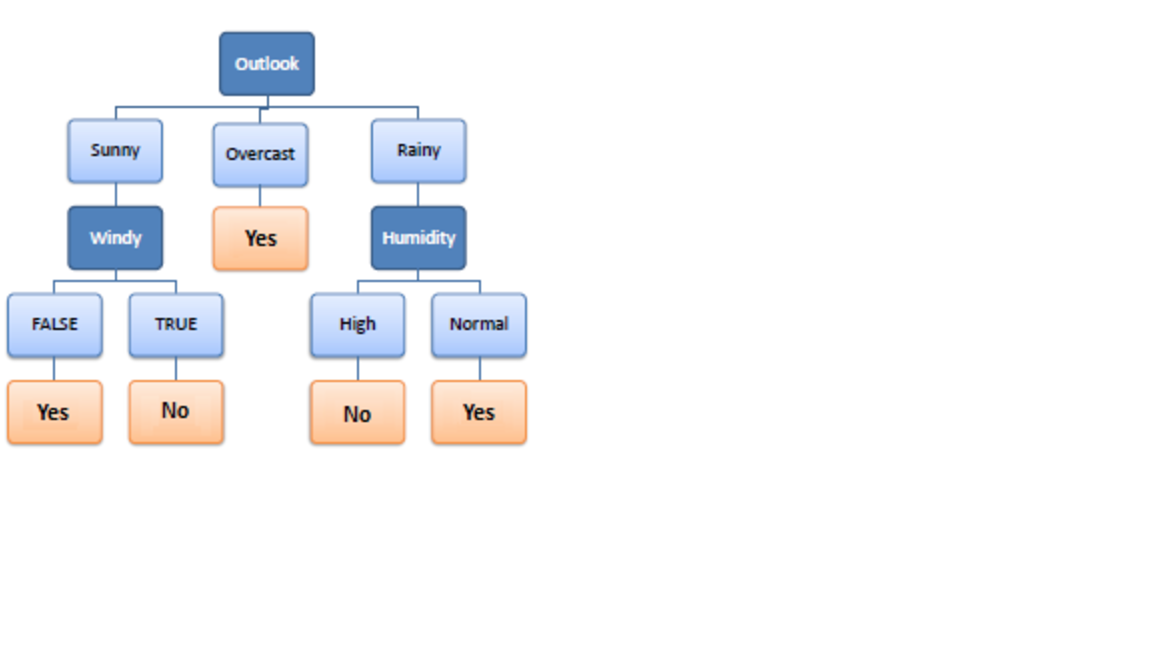
\includegraphics{decisiontree}
    \label{fig:decisiontree}
\end{figure}

\section{SimForest}

Extracting a multidimensional embedding from the similarity matrix could be a possible solution to this problem of random forests. The authors have proposed the construction of random forests directly with similarity matrices without accessing multidimensional representation of the data. This approach is refered to as simForest, which corresponds to the fact that it is similarity forest. SimForest assumes that the data is embedded in some theoretical multidimensional space, and then use the similarities for computing the the coordinates of data points along 1-dimensional projections. Simforests creates these 1-dimensional projections by sampling pairs of points belonging to different classes, and then for each pair projecting the remaining points along the theoretical multidimensional direction representing the line joining the pair.  \\


\section{Problem Definition}
SimForest assumes that there is a set of \textit{n} objects denoted by $O_1$...$O_n$. These n objects can be of any data type, and most cases, the specific object type does not need to be known as long as it is possible to compute a similarity value between them. The similarity between $O_i$ and $O_j$ is denoted by $S_ij$, and it may not necessarily be available up front to the algorithm.For example, in the time-series domain, s domain-specific similarity function may be used. In such cases, the similarity between objects are computed on the fly as needed by the algorithm.\\

\section{THE SIMFOREST ALGORITHM}
The theoretical embeddings are denoted as ${\bar{X}_1}$...${\bar{X}_n}$. ``direction'' in the data space refers to the the theoretical embedding  ${\bar{X}_1}$...${\bar{X}_n}$. The method constructs each decision tree in the similarity forest in a top-down fashion by using recursive splits. This approach is similar to the traditional random forests approach. SimForest algorithm samples directions from the original space just as traditional random forests samples features for splitting. The pairs of objects can be sampled in one or two ways:\\
\begin{itemize}
\item The pairs are randomly selected without taking into consideration the class label.
\item Randomly selected pairs always belong to different classes. This implies that the object in the pairs is randomly selected, whereas the second is selected from objets belonging to a different class.
\end{itemize}
 
Construct each tree in the forest using sampled pairs of points and splitting using similarity values.\\
A pair of objects $O_i$ and $O_j$ that define the direction of the split.\\
Consider an object $O_k$ that needs to be projected along this direction. The unit direction of the embedding is given by\\

$$\frac{\overline{X_{i}}-\overline{X_{j}}}{ \parallel \overline{X_{i}}-\overline{X_{j}} \parallel}$$
 $$ P(\overline{X_{k}})=(\overline{X_{k}}-\overline{X_{i}})\frac{\overline{X_{i}}-\overline{X_{j}}}{ \parallel \overline{X_{i}}-\overline{X_{j}} \parallel}$$
 $$P(\overline{X_{k}})= \frac{\overline{X_{k}} \cdot \overline{X_{j}}-\overline{X_{k}} \cdot \overline{X_{i}} -\overline{X_{i}} \cdot \overline{X_{j}}+\overline{X_{i}} \cdot \overline{X_{i}}}{\parallel \overline{X_{i}}-\overline{X_{j}} \parallel} $$
 $$=\frac {S_{kj}-S_{ki}-S_{ij}+S_{ii}}{\parallel \overline{X_{i}}-\overline{X_{j}} \parallel}$$
 $$=\frac {S_{kj}-S_{ki}-S_{ij}+S_{ii}}{\sqrt{S_{ii}+S_{jj}-2S_{ij}}}$$
 $$P(\overline{X_{k}})=A\cdot (S_{kj}-S_{ki})+B$$
 $$GQ(N_{1},N_{2})=\frac {n_{1}G(N_{1})+n_{2}G(N_{2})}{n_{1}+n_{2}}$$

\noindent Construct each tree in the forest using sampled pairs of points and splitting using similarity values.


\subsection{Testing Phase}
The testing phase uses an identical approach to project the test points on the line defined by the pairs of training points at each node. The testing phase is as follows:

\begin{itemize}
\item If ($O_i$, $O_j$) is the defining pair of objects for a given node, then the value of $S_{ki}$- $S_{kj}$ is computed for the test object $O_k$.
\item The stored split point (say $\alpha$) is used to determine which path in the decision tree to follow depending on whatever on whether or not $S_{ki}$- $S_{kj} \leq  \alpha$ 
\item This step is performed for each node on the path on the tree, until the object $O_k$ is assigned to a leaf node.
\item The label of the leaf is reported as the prediction
\end{itemize}
\section{Implementation}
Our goal for this project was to implement the SimForest algorithm and compare it with the rndom forests and Support Vector Machines (SVM) and validate that the SimForest model wors with a non multidimensional as well as a multidimensional data sets.\\
\subsection{Data Preprocessing}
The first step we took in this implementation is the data exploration and data preprocessing. We got the data sets from \url{https://www.csie.ntu.edu.tw/~cjlin/libsvmtools/datasets/binary.html#breast-cancer}. We had to explore the data in order to understand the data sets we were working with. After exploration, we observed missing values. We first converted all strings to \textit{NaN} and used \textit{sciklearn Imputer} package to replace missing values with mean and normalized the data set to zero mean and unit variance. After handling missing value, we use sklearn \textit{Label Encoder} to convert categorical variables into numerical variables where variables such as benign and malignant in the breast cancer data set was replaced with \textbf{0}  and \textbf{1}  respectively. The code snippet in listeng 1 explains how we apply these python packages.

\begin{lstlisting}[caption={Preprocessing code},label={lst:label},language=python]


dataset = dataset.convert_objects(convert_numeric=True)

X1 = dataset.iloc[:, :-1].values
y1= dataset.iloc[:, 13]

from sklearn.preprocessing import Imputer
imputer = Imputer(missing_values = "NaN", strategy ="mean", axis = 0)
imputer = imputer.fit(X1[:, 0:13])   
X1[:, 0:13] = imputer.transform(X1[:, 0:13])
y1=np.array(y1)
\end{lstlisting}
\subsection{Model Fitting}
After getting our data sets ready, the next step was the model fitting. There is no package for the similarity forest algorithm. We implemented this algorithm from scratch. One of the things we achieved in this project was to write this algorithm as a package. We hope that this package will benefit other researchers and also showcase the power of this SimForest algorithm to the world. Writing this algorithm made it easy for us to call the method on our train and target features.\\

\noindent For Support Vector Machines and Random Forests, we used the \textit{sciklearn} model and called both methods on our train and target features. We did not try to implement the algorithm from scratch because the packages were already available.

\begin{lstlisting}[caption={Model Fitting code},label={lst:label},language=python]
 cancer = load_breast_cancer() 
    X_train_dia, X_test_dia, y_train_dia, y_test_dia = 
    train_test_split(cancer.data, cancer.target, test_size=0.2, random_state=0)
    
    rf = RandomForestClassifier()
    rf.fit(X_train, y_train)
    rf_pred = rf.predict(X_test)
    
    sf1 = SimilarityForest(n_estimators=10, n_axes=1)
    sf1.fit(X_train_dia, y_train_dia)

    sf1_pred = sf1.predict(X_test_dia)
    sf1_prob = sf1.predict_proba(X_test_dia)
    
    lr = LogisticRegression(random_state=0)
    lr.fit(X_train, y_train)
    lr_pred=lr.predict(X_test)
    
\end{lstlisting}

\section{EVALUATION AND RESULTS}

\begin{lstlisting}[caption={Model Evaluation with Accuracy},label={lst:label},language=python]
dict_acc_1={'Simlarity forest ':accuracy_score(y_test, sf_pred), \
    'Random forest ':accuracy_score(y_test, rf_pred), 'Svm ':accuracy_score(y_test, svm_pred),\
    'Logistic regression ':accuracy_score(y_test, lr_pred)}
    df_acc_1=pd.DataFrame(list(dict_acc_1.items()))
    df_acc_1.columns=['Model','Accuracy']
    df_acc_1.Accuracy=df_acc_1.Accuracy*100
\end{lstlisting}
Determining the accuracy of a model is based on various evaluation metrics. An evaluation matrix is used to explain the performance of a model. Since the goal of this project is to compare SimForerest with other models, it is vital that we evaluate the performance of these models.\\

\noindent For this project, we have used accuracy to evaluate the performance of these models. We plotted the various models with accuracy.

\begin{figure}[H]
    \caption{Random Data}
    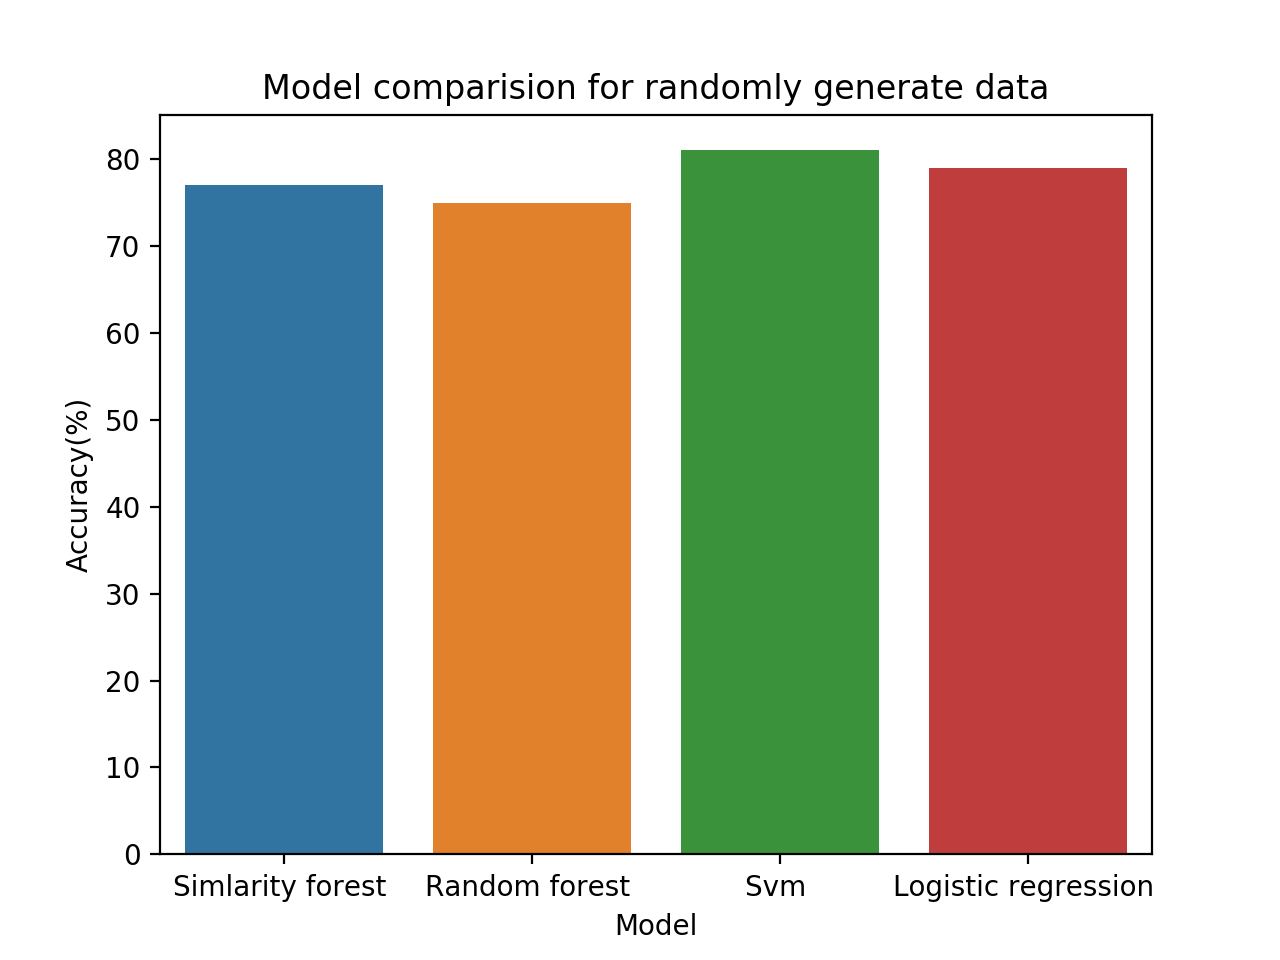
\includegraphics{randomdata}
    \label{fig:randata}
\end{figure}

\begin{figure}[H]
    \caption{Heart Data}
    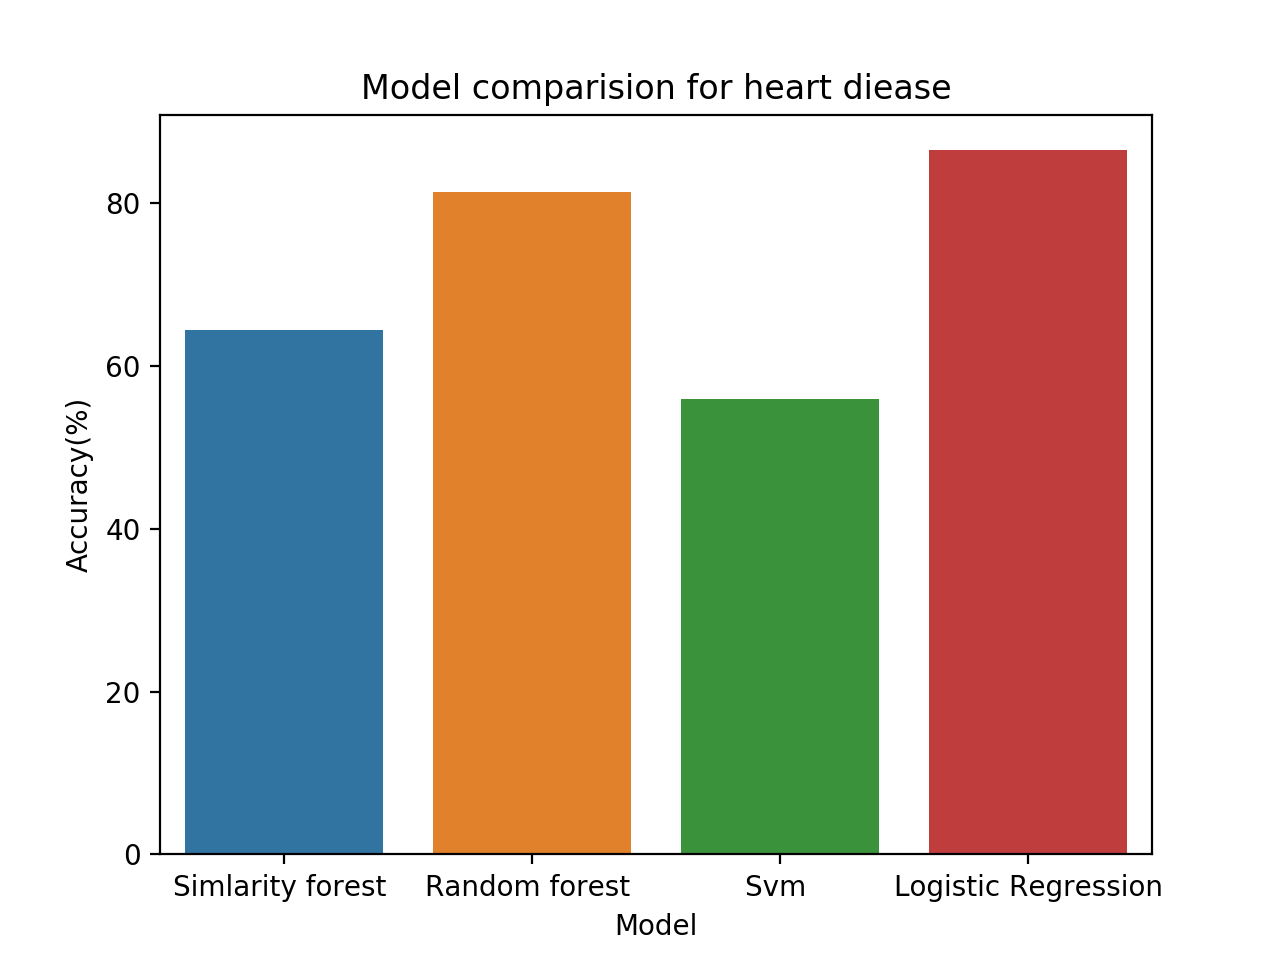
\includegraphics{heartdata}
    \label{fig:heartdata}
\end{figure}

\begin{figure}[H]
    \caption{Breast Cancer Data}
    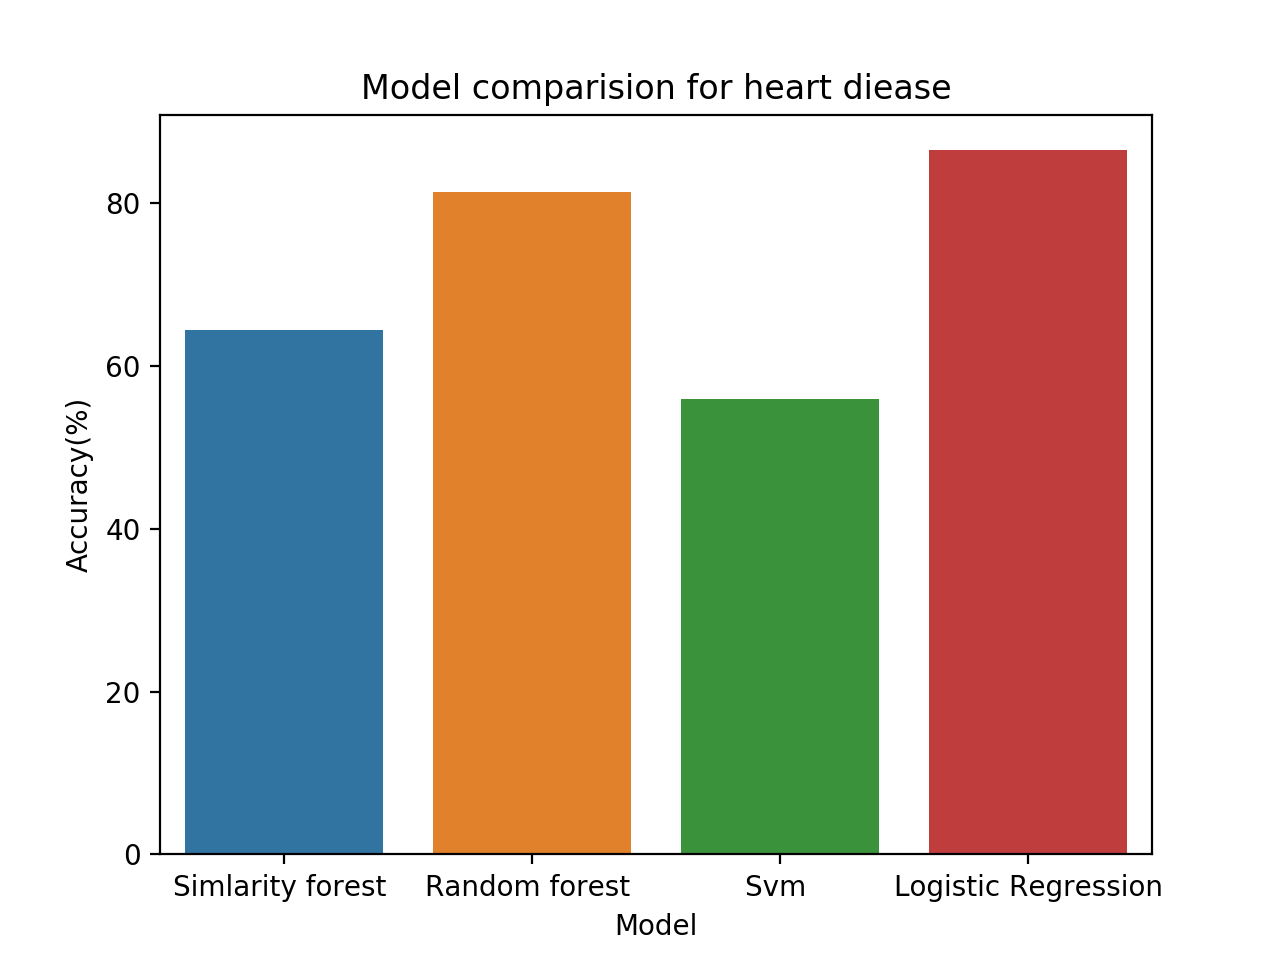
\includegraphics{heartdata}
    \label{fig:breastdata}
\end{figure}

\noindent Figure ~\ref{fig:randata} shows the result of the four different models we implemented on a randomly generated data set. In this data set, the SVM performed better than the other models. Although the difference is not much, this explains how linear models perform in a randomly generated data set against non-linear model.\\

\noindent For the the next data set, the heart disease data set, 
Figure ~\ref{fig:heartdata} shows the accuracy of various models on the heart disease data set. In the paper, the authors did not test Logistic Regression. This is our extra credit. SVM has the least accuracy while Logistic Regression has the highest accuracy. Random forests outperformed SimForest and the reason is because this is a multidimensional data set.\\

\noindent This last data set we used to evaluate this model is the breast cancer data set. Figure ~\ref{fig:breastdata} shows the accuracy of the models. Again, SVM performed least while Logistic regression performed better that the other models. We would like to state that the authors did not test Logistic Regression with the other models.\\

\section{CONCLUSION}
We have used two different data sets and a randomly generated data set to test the performance of the Similarity Forest, Random Forests, Support Vector Machines and Logistic Regression models. The authors only tested SimForest, Random Forests and SVM models. Since SimForest and Random Forests are both non-linear models, we decided to also test with a non-linear Logistic Regression model.\\

In our result, we saw that the SinForest and Random Forests performed better that the SVM model. However, Logistic Regression performed better than the other non-linear models and the linear (SVM) as well. 



\section{EXTRA CREDIT}

Random Forests and SimForest are both non-linear machine learning models. In the paper, the authors compared Support Vector Machines (SVM) with Random Forests and SimForest. Since SVM is a linear model, for the extra credit, we decided to test SimForest with a non-linear model. We wanted to see how a different non-linear model will perform with SimForest and Random Forests. The Random Forests is a non-linear model and SimForest is an adaptation of the Random Forests. We have followed the same steps we took during the original model implementation (data exploration, preprocessing, model fitting and evaluation) for the extra credit. We have also observed that the Logistic Regression Model performed better than the Random Forests and SimForest model. This is interesting because the Random Forests is said to be one of the most effective and successful machine learning algorithms. \\

\noindent Time did not allow us to investigate this observation further.\\

 

\noindent For the second extra credit, we have applied similarity forest on a different data set. Since the goal of our project is to compare the accuracy of the models, it is also important to check the performance of these models on a different data set. The heart disease data set is for the extra credit.\\


\newpage



% TABLES
\begin{thebibliography}{}
\bibitem{Sathe, Saket and Aggarwal, Charu C} Saket Sathe and Charu C. Aggarwal  2017,
      Similarity forests,
     Proceedings of the 23rd ACM SIGKDD International Conference on Knowledge Discovery     and Data Mining
      (ACM) 395-403

\end{thebibliography}



\end{document}

